% Copyright 2021 Joel Feldman, Andrew Rechnitzer and Elyse Yeager, except where noted.
% This work is licensed under a Creative Commons Attribution-NonCommercial-ShareAlike 4.0 International License.
% https://creativecommons.org/licenses/by-nc-sa/4.0/

\documentclass[10pt]{beamer}

 %%%%%%%%%%%%%%%%%%%%%%%%%
 %%%%%%%%%%%%%%%%%%%%%%%%%
 %%%%%%%%%%%%%%%%%%%%%%%%
\usepackage{header100}


\begin{document}

%----------------------------------------------------------------------------------------

%----------------------------------------------------------------------------------------
\begin{frame}{CLP-1 Lecture Slides}
The slides in this folder are written to correspond to \href{https://secure.math.ubc.ca/~CLP/CLP1/}{CLP-1 by Feldman, Rechnitzer, and Yeager}. The slides and their source files can be found online at \url{https://github.com/ecyeager/CLP1Slides}.
\vfill

CLP-1 lecture slides are Copyright 2021 Joel Feldman, Andrew Rechnitzer and Elyse Yeager, except where noted.
They are licensed under a Creative Commons Attribution-NonCommercial-ShareAlike 4.0 International License.
\begin{center}

\includegraphics[height=7mm]{Clipart/CC}
\end{center}
\url{https://creativecommons.org/licenses/by-nc-sa/4.0/}
 \end{frame}
%----------------------------------------------------------------------------------------

%----------------------------------------------------------------------------------------
\section{Files}
\frame{\tableofcontents[currentsection]}
%----------------------------------------------------------------------------------------
%----------------------------------------------------------------------------------------
\begin{frame}{Versions}
Most slides have three versions.
\begin{description}
\item[beamer] The beamer mode is used to generate slides that will be used in class. These have all the ``clicks" (pauses inside frames) and space to write solutions to questions. Solutions to most questions are also included.
\item[handout] The handout mode is used to generate slides that students can access before lecture and use to take notes. Most clicks are suppressed. Solutions to questions are also suppressed, so students can work in class without spoilers.
\item[prep] There are occasional notes with scripts for lecture, notes on common student difficulties, and explanations of otherwise-confusing slides. You wouldn't want to display them in class, but they might be helpful to look at when you're preparing.
\end{description}
\end{frame}
%----------------------------------------------------------------------------------------
\begin{frame}{Organization}
PDFs can be found in the \texttt{pdfs} folder, while the folder \texttt{src} has their source files.
\vfill

Slides for a single section are compiled in files named with the section, a short description, and the version type. (For example, \texttt{1\_3LimitOfFunction\_Handout.pdf} is the handout version of Section 1.3, The Limit of a Function.) 

\vfill
The slides are also arranged into batches corresponding to roughly one week of lecture each, for a 12-week class. The filenames give the week number, a description, the range of associated sections, and the version.
(For example, \texttt{W1Limits\_1\_1-1\_4\_Prep} is the prep version of Week 1, which includes sections 1.1-1.4, covering limits.) 
\vfill
\end{frame}
%----------------------------------------------------------------------------------------
\begin{frame}{Irregularities}
Sections 1.7 and 1.8 are marked as optional. They do have section PDFs, but are not included in any of the weekly batches. In the slides, Section 1.8 is meant to be covered before Section 1.7.\vfill

Sections 2.4-2.6 are closely related. They are all included in the section marked 2.4. That is why there are no sections marked 2.5 or 2.6.\vfill
\end{frame}
%----------------------------------------------------------------------------------------
\begin{frame}{Miscellaneous Files}

The file StudentWorkbook.pdf has slides for the whole course, with answers removed, formatted for printing. Students who wish to write on paper (rather than annotating PDFs on a tablet) can print out the file and have a workbook to follow for the entire semester.\vfill

The file Review.pdf has a list of questions from Chapters 1-3.
\vfill

\end{frame}
%----------------------------------------------------------------------------------------
\section{Compiling}
%----------------------------------------------------------------------------------------
\begin{frame}{Compiling Options}
There are many files, so we included options for compiling them efficiently. The files can be compiled using pdflatex (in the usual way you probably compile LaTeX); using a Python script to compile many files in one go; and using a Python script with parallel processing and latexmk to quickly compile many files in one go.
\end{frame}
%----------------------------------------------------------------------------------------
\begin{frame}{Compiling Without Python}
In the folder \texttt{src}, you'll find a list of .tex files corresponding to each section, each weekly batch, StudentWorkbook, ReadMe, and Review. 
\vfill

To change the version of the file (beamer, handout, prep), change which headers are commented out in the .tex file.

\vfill

Individual .tex files are compiled with pdflatex. From the \texttt{src} folder, \texttt{pdflatex --output-directory ../pdfs  <filename> } will put the PDF into the folder \texttt{pdf}.
\end{frame}

%----------------------------------------------------------------------------------------
\begin{frame}{Compiling With Python}
Running \texttt{buildPDFs\_parallel.py} or \texttt{buildPDFs\_slow.py} will compile the slides and sort the PDFs into their directory. By default, they will compile all versions of all files. This may take a long time: each (non-optional) section is included in beamer, handout, and prep versions of single sections and weeks, as well as the student handout file, so most sections are compiled 7 times.\vfill

Both start with options to specify which files should be compiled. Set each variable to True or False in the .py file.\vfill
\begin{tabular}{lcl}
\textbf{variable} &\textbf{ value} & \textbf{behaviour}\\\hline
\texttt{print\_beamer} & True & print beamer versions of  slides\\
 & False & do not print beamer versions
\\\hline
\texttt{print\_handout} & True & print handout versions of  slides\\
 & False & do not print handout versions
\\\hline
\texttt{print\_prep} & True & print prep versions of  slides\\
 & False & do not print prep versions
\\\hline
\end{tabular}
\end{frame}

%----------------------------------------------------------------------------------------
\begin{frame}

\begin{tabular}{lc l}
\textbf{variable} &\textbf{ value} & \textbf{behaviour}\\\hline
\texttt{print\_sections} & False & print no single sections\\
 & True & print all single sections from the list\\
 \hline
\texttt{print\_weeks} & False & print no weekly batches\\
 & True & print all weekly batches from the list\\
 \hline
\texttt{print\_readme,} 
&False & \parbox[t]{0.55\textwidth}{\raggedright do not print the corresponding file (ReadMe, Review, or  StudentWorkbook)}\\
\parbox[t]{0.2\textwidth}{\texttt{print\_review,\\print\_studentworkbook}}
&True & print the corresponding file
\\\hline
\parbox[t]{0.2\textwidth}{\texttt{delete\_aux} \\ (in parallel file only)}& False &  \parbox[t]{0.55\textwidth}{all auxiliary files (.aux, .log, .toc, .nav, etc.) are kept}\\
 & True & \parbox[t]{0.55\textwidth}{all files that are generated when the program runs will be deleted (except the resulting .pdf). }
 \\ \hline
\end{tabular}
\end{frame}

%----------------------------------------------------------------------------------------
\begin{frame}
Below the compilation choices are lists of sections and weeks. These are lists of exactly which sections and which weeks to compile. If you would like to omit some (but not all) of these files, comment them out of the list.\vfill

If you have already set \texttt{print\_sections=False} or \texttt{print\_weeks=False}, there is no need to comment out the sections or weeks. None of them will be compiled.
\vfill

There are no further customization options after the lists of sections and weeks.
\end{frame}

%----------------------------------------------------------------------------------------
\begin{frame}{{BuildPDFs\_slow.py} vs. {BuildPDFs\_parallel.py}}
\texttt{BuildPDFs\_parallel.py} uses parallel processing to speed things up. It also uses latexmk, which requires Perl to be installed. The parallel file has the option to delete auxiliary files. You only need to run \texttt{BuildPDFs\_parallel.py} once.
\vfill

\texttt{BuildPDFs\_slow.py} compiles files one-at-a-time using pdflatex. It is slower, but might work out-of-the-box on more machines -- for example, Windows machines without Perl installed. The repository does not track auxiliary files, so using this option you will initially have to compile twice to generate the navigation bars in the header and to make the internal references work.
\end{frame}

%----------------------------------------------------------------------------------------
\section{Philosophy}
%----------------------------------------------------------------------------------------
\begin{frame}{A Note on Repetition}
I have observed in my 100-level classes the usefulness of repeated concrete examples. At this stage in their development, many students have a hard time applying theorems in the way mathematicians usually want to state them, but are adept at noticing patterns.\vfill

This observation lies in the background of many of the decisions I made in putting together these slides. In this document, you'll see that I often help myself keep track of where I am in a repetitive sequence. It may seem silly or boring, but in my own experience, I have found the repetition to be useful.
\end{frame}
%----------------------------------------------------------------------------------------
\begin{frame}{Active Learning}
Another technique I often employ in introductory classes is to pepper my lectures with opportunities for students to engage on their own (and with their neighbours) with the material. \vfill

There will sometimes be several questions visible on the same slide. In class, I encourage students to work on the first one or two questions, and to move on to the others only if they are ``super speedy" and finish the target question(s) early. This balances out different student needs. Those who need more time can have it, because those who need less time are still able to stay engaged.
\end{frame}
%----------------------------------------------------------------------------------------
\begin{frame}{Posting Notes}
What exactly to give students access to is a very personal decision.  I do not know the best solution. Students who do not have access to lecture notes may be more motivated to synthesize content in their own words. Students who do have access to lecture notes may feel less pressure during class. 
\vfill

My personal practice in 100-level courses is to give students a handout without solutions to write on in class, and post the full slide version with solutions online after class. Providing the handout means that students don't spend time and energy copying down things like definitions that are easily found in the textbook. Withholding solutions during class enables the active learning described on the previous slide. Letting students know that solutions will be posted later encourages students to copy down only what seems important to them in the moment, rather than trying to reproduce every line exactly.
\end{frame}
%----------------------------------------------------------------------------------------
\begin{frame}{Common Mistakes}
When addressing common misconceptions, rather than saying ``it's common to make mistake $X$...," I'll give students a multiple-choice question where $X$ is an option. I think the students who go out on a limb and select $X$ are more likely to remember that it's incorrect when they've been primed by that gentle bit of chagrin. I like to follow these with a second round of questions, which allows students to claim the new knowledge for themselves, rather than sitting with their embarrassment. This is also an opportunity to promote growth mindset.
\end{frame}
%----------------------------------------------------------------------------------------
\begin{frame}{Attribution}
Attribution information is generally found at the end of each file, if the file includes work from other sources.
\end{frame}

%%----------------------------------------------------------------------------------------
%----------------------------------------------------------------------------------------
\section{Interpreting the visual cues}
\frame{\tableofcontents[currentsection]}
%----------------------------------------------------------------------------------------
%----------------------------------------------------------------------------------------
\begin{frame}{Lecturer Cues}
The lower right-hand corner of the slides  holds icons that will be useful for the lecturer but that are not necessary for students to pay attention to. These are meant to be relatively unobtrusive. They do not appear in handout mode.
\vfill

This slide has a box letting you know that the current question has its answer written in. If you click too far, you may give it away.
\AnswerYes
\end{frame}
%----------------------------------------------------------------------------------------
\begin{frame}{No answer}
This slide has the opposite cue: the answer to the current question does \textit{not} appear on the slides. 
\AnswerNo
\end{frame}
%----------------------------------------------------------------------------------------
\begin{frame}{More space}
The notebook icon in the corner tells you that there is more room on the next slide.
This is used when a slide has a question with little room after it to work.
\vfill

Usually, the question is sharing the slides with a theorem or a similar example.
You can see the problem together with the other content in order to talk about the problem before you write anything down, or to give students a chance to start working on their own. When it's time to work the problem on a tablet, you can advance to the next slide, hiding the extra information to open up space.
\MoreSpace
\end{frame}
%----------------------------------------------------------------------------------------
\begin{frame}{Question Set}
The staircase status bar is used for sets of related questions. The status bar on this slide shows the 4th of 5 questions in a set.\vfill
\QuestionBar{4}{5}

I overload my slides with questions to make sure I don't run out of content. \alert{I do not generally present every single problem in a file.} When there's a large set of similar problems, I choose the ones I have time for.
\end{frame}
%----------------------------------------------------------------------------------------
\begin{frame}{Status Bar}
These frames have a  flipbook-style animation. The status bar in the corner tells you where you are in that flipbook, so you know when to stop clicking.

\begin{center}
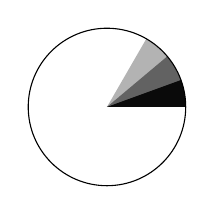
\begin{tikzpicture}
\draw (1,0) arc (0:360:1cm);
\foreach \x in {1,2,3}{
	\onslide<\x>{\fill[opacity=0.9/\x](1,0) arc(0:20*\x:1cm)--(0,0)--cycle;}
	}
\end{tikzpicture}
\end{center}
\StatusBar{1}{3}
\end{frame}
%----------------------------------------------------------------------------------------
\begin{frame}{Now You}
\NowYou The brain-training icon indicates a question for students to work on alone or in groups.
(Since this is information for students as well as instructors, the icon is not stashed in the lower right-hand corner.)
\vfill

In a first-year class, it may take time to establish a culture where students work earnestly on in-class problems. I like to emphasize that students are building skills. Building a skill requires not just understanding but practice.
\end{frame}
%----------------------------------------------------------------------------------------
\begin{frame}{Unobtrusive Notes}
\unote{ $\rightarrow$ Here, in the left-hand corner, by the page number $\leftarrow$}
References to the text are sometimes put next to the page number. 
Content on the slides is similar, but usualy not identical, to the reference. The references can help you judge which part of the text corresponds to the current slide.
\vfill

Keen students can investigate the references in the text if they want a longer written explanation, or a similar example to practice on. For that reason, these show up the handouts as well as in beamer mode. 
\end{frame}
%----------------------------------------------------------------------------------------
%----------------------------------------------------------------------------------------
\begin{frame}
If you just want to use the slides as they are, you can stop here. 
\vfill
The remaining sections describe how to use the custom macros, and are only necessary if you intend to \alert{edit} the slides.
\end{frame}

%----------------------------------------------------------------------------------------
%----------------------------------------------------------------------------------------
\section{Using question and answer macros}
\frame{\tableofcontents[currentsection]}
%----------------------------------------------------------------------------------------
%----------------------------------------------------------------------------------------
\begin{frame}[t]{Who Does a Question}

\NowYou The command \texttt{\textbackslash NowYou} places a visual cue that the written exercise is meant to be done by students, rather than the lecturer. There is no other formatting.\vfill

The command includes a citation for the brain training icon, which will show up when you run \texttt{\textbackslash LastPage} to include the attribution page.
\end{frame}

%----------------------------------------------------------------------------------------
\begin{frame}[fragile]{Printing Answers}
You can set the toggle printsolutions to true or false in the preamble. \vfill
\begin{verbatim}
\settoggle{printsolutions}{true}
\settoggle{printsolutions}{false}
\end{verbatim}\vfill

If you set the toggle to false, the answers will not be printed.  The toggle is automatically set to false in handout mode, and to true in beamer mode.\vfill

The syntax to use it directly is:\vfill
\begin{verbatim}
\iftoggle{printsolutions}{<A>}{<B>}
\end{verbatim}\vfill
where $<$A$>$ will show if the toggle is set to true, and $<$B$>$ will show otherwise.
\end{frame}
%----------------------------------------------------------------------------------------
\begin{frame}
You can use \texttt{\textbackslash answer\{$<$A$>$\}} as a shortcut for \texttt{\textbackslash iftoggle\{printsolutions\}\{$<$A$>$\}\{\}}. That macro does nothing else.\vfill


The printsolutions toggle also affects the commands: \texttt{\textbackslash SetQuestion\{\}}, \texttt{\textbackslash SetAnswer\{\}, \textbackslash AnswerYes,  \textbackslash AnswerNo}, and \texttt{\textbackslash AnswerSpace} \vfill

\end{frame}
%----------------------------------------------------------------------------------------
%----------------------------------------------------------------------------------------
\begin{frame}{Sets of Questions}
Sometimes there are sets of questions on a particular topic. You can put these inside a \texttt{QuestionSet} environment,  then give questions inside \texttt{\textbackslash SetQuestion\{\}} and  answers inside \texttt{\textbackslash SetAnswer\{\}}. The answers will be shown or hidden according to the printsolutions toggle. Since handout mode sets the printsolutions toggle to false, answers are automatically hidden in handouts.
\vfill

Each question (in both modes) and each answer (in beamer mode) will show up on one frame. Question and answer staircase status bars will be printed accordingly. If the set has more than about 7 questions, these bars might overrun the page.
\end{frame}
%----------------------------------------------------------------------------------------

%----------------------------------------------------------------------------------------
\begin{frame}{More Flexible Sets of Questions}
The \texttt{QuestionSet} environment takes care of a lot of things for you (like making the items show up on different slides in a handout, and counting how many there are total). The trade-off is that it might be too restrictive. It can only be in one frame environment, for example, and each question will be on a new overlay.
\vfill
A more general way of getting the staircase Q\&A status bar is to use \texttt{\textbackslash QuestionBar\{$<$a$>$\}\{$<$b$>$\}}
and \texttt{ \textbackslash AnswerBar\{$<$a$>$\}\{$<$b$>$\}}. This will put a staircase status bar showing $<$a$>$ of $<$b$>$ total. You'll probably want to wrap these in an \texttt{\textbackslash only} overlay specification to control where they show up. Unlike \texttt{QuestionSet}, the total size of the status bar is fixed, so you don't have to worry about overrunning margins.\vfill

\texttt{\textbackslash QuestionBar\{2\}\{7\}}
\QuestionBar{2}{7}
\end{frame}

%----------------------------------------
\begin{frame}
\AnswerYes
 \texttt{\textbackslash AnswerYes} and  \texttt{\textbackslash AnswerNo} place answer boxes in the lower right-hand corner. To have them show up on only certain slides, you must use \texttt{\textbackslash only}, rather than \texttt{\textbackslash onslide}.\vfill
 

 The answer boxes can affect the alignment of a slide.   \texttt{\textbackslash AnswerSpace}  avoids jarring text displacement between overlays by making an invisible box of the same size. (It makes \texttt{\textbackslash only} behave more like \texttt{\textbackslash onslide}.)
\end{frame}
%----------------------------------------------------------------------------------------
%----------------------------------------
\section{Using other macros}
\frame{\tableofcontents[currentsection]}
\begin{frame}[t,fragile]
Lecturer cues in the corner won't be placed correctly if you have \verb|\centering| on the page, so use \verb|\begin{center} \end{center}| instead, and put the commands outside.
\vfill
The macros in this category are:
\begin{itemize}
\item \verb|\MoreSpace|
\item \verb|\StatusBar|
\item \texttt{QuestionSet} environment with \verb|\SetQuestion| and \verb|\SetAnswer| 
\item \verb|\QuestionBar, \AnswerBar|
\item \verb|\AnswerYes, \AnswerNo, \AnswerSpace|
\end{itemize}
\end{frame}
%----------------------------------------------------------------------------------------
%----------------------------------------------------------------------------------------
\begin{frame}[t]{Slide Clicks}
The command \texttt{\textbackslash StatusBar\{$<$a$>$\}\{$<$b$>$\}} will place a small status bar in the lower-right hand corner of the frame, starting at slide number $<$a$>$ and ending at slide number $<$b$>$.\vfill
\StatusBar{1}{1}
\end{frame}
%----------------------------------------------------------------------------------------

\begin{frame}[t]{Map of Contents}
The mindmap tables of contents aren't automatically generated from the sections in a document. Rather, they are saved in the file \texttt{header\_maps.sty}.\vfill

Each chapter has its own map. You can highlight any number of sections in a chapter. Since numbers don't work in TeX as variable names, sections are labeled with letters: 1 is a or A, 2 is b or B, etc. There is one exception: to avoid re-defining \texttt{\textbackslash bf}, in Chapter 2, sections 6 and up are off by one in their labels. So section 2.5 is \texttt{\textbackslash be}, and section 2.6 is \texttt{\textbackslash bg}.
\vfill

The command \texttt{\textbackslash mapofcontentsA\{\textbackslash ac,\textbackslash ab}\} will show the map of contents for Chapter 1 (that's the ``A" in the command itself) with sections 1.3 and 1.2 highlighted (that's the list in the argument). \\

The command \texttt{\textbackslash mapofcontentsC\{\}} will show the map of contents for Chapter 3 (that's the ``C" in the command itself) with no sections highlighted (since the argument is empty).\\

\end{frame}
%----------------------------------------------------------------------------------------

\begin{frame}[fragile]{Referencing the Textbook}
\verb|\eref{text}{<label>}| and \verb|\eref{prob}{<label>}| allow you to reference labelled items in the textbook and problem book, respectively. The folder XR has the aux files from these texts. When the texts are updated, copying the new aux files to that folder will make all the references in the slides update when they are re-compiled.
\vfill

\texttt{\textbackslash unote\{$<$content$>$\}} will put $<$content$>$ next to the footline page number. I have used this exclusively to reference the textbook and problem book.
\unote{$<$content$>$}
\end{frame}

%----------------------------------------------------------------------------------------
\begin{frame}[t]{Attribution}

The index is used to cite copyrighted content. The standard format for setting up a citation of an image is:


\texttt{\footnotesize\textbackslash index\{\textbackslash includegraphics[height=5mm]\{$<$file.png$>$\} $<$picture title (link)$>$ by $<$artist (link)$>$ is licensed under $<$license information (link)$>$\}
}

\vfill

The command \texttt{\textbackslash LastPage} prints an index of copyrighted works included in the file so far. If none have been cited with the \texttt{\textbackslash index} command, it will print nothing.\vfill

\texttt{\textbackslash  CCBYtwo , \textbackslash CCBYthree \textbackslash  CCBYNCNDfour,} and \texttt{\textbackslash CCBYNCSAtwo} display and link to their respective licenses.
\end{frame}

%%----------------------------------------------------------------------------------------
\begin{frame}{Colour Scheme}
The following named colours are used in graphics. \vfill
\begin{tikzpicture}
\foreach \x in {1,2}
{
	\draw[white] (\x*1.5,1) node[shape=circle, fill=C\x, minimum size=1cm]{C\x};
	\draw[white] (\x*1.5,3) node[shape=circle, fill=M\x, minimum size=1cm]{M\x};
	\draw[white] (\x*1.5,5) node[shape=circle, fill=W\x, minimum size=1cm]{W\x};}
\foreach \x in {3,4,5}
{
	\draw (\x*1.5,1) node[shape=circle, fill=C\x, minimum size=1cm]{C\x};
	\draw (\x*1.5,3) node[shape=circle, fill=M\x, minimum size=1cm]{M\x};
	\draw (\x*1.5,5) node[shape=circle, fill=W\x, minimum size=1cm]{W\x};}
\draw (0,1)node{cool}; \draw (0,3)node{mixed}; \draw (0,5)node{warm};
\end{tikzpicture}

\end{frame}
%----------------------------------------------------------------------------------------
%----------------------------------------------------------------------------------------
\LastPage
%----------------------------------------------------------------------------------------
%----------------------------------------------------------------------------------------
\end{document}
%----------------------------------------------------------------------------------------
